\documentclass[a4paper,12pt]{article}

\usepackage{fancyhdr}
\usepackage{lastpage}
\usepackage{amsmath}
\usepackage{tikz}
\usepackage{amsfonts}
\usepackage{graphicx}

\newcommand{\F}[2]{\ensuremath{\frac{#1}{#2}}}
\newcommand{\V}[1]{\ensuremath{\vec{#1}}}
\newcommand{\Q}[1]{\newpage \section*{#1}}
\newcommand{\vel}[1]{\overset{.}{#1}}
\newcommand{\acc}[1]{\overset{..}{#1}}
\newcommand{\LP}{\left(}
\newcommand{\RP}{\right)}

\pagestyle{fancy}
\lhead{Samuel Loomis}
\setlength{\headheight}{15pt}
\chead{Classical Mechanics Homework 6}
\rhead{11/11/13}
\lfoot{}
\cfoot{\thepage\ of \pageref{LastPage}}
\rfoot{}

\begin{document}

\section*{Problem 1: Taylor 7.16}
Write down the Langrangian for a cylinder (mass $m$, radius $R$, and moment of inertia $I$) that rolls without slipping straight down an inclined plane which is at an angle $\alpha$ from the horizontal.  Use as your generalized coordinates the cylinder's distance x measured down the plane from its starting point.  Write down the Lagrange equation and solve it for the cylinders acceleration $\acc{x}$. Remember that $T= \F{1}{2}mv^2+\F{1}{2}I\omega^2$, where $\V{v}$ is the velocity of the center of mass and $\V{\omega}$ is the angular velocity.

The potential energy of the cylinder drops as the cylinder moves along the plane.  The potential energy at any time is equal to the mass times the acceleration of gravity times its height.  If the initial potential energy is set to 0 at the initial position of x, as x increases, the height must decrease.\\ \\
\begin{figure}[h]
\centering
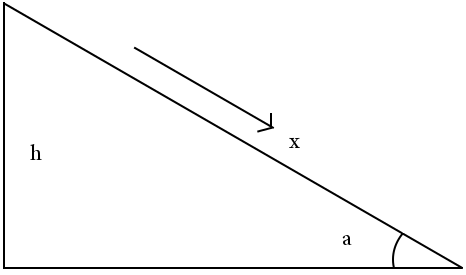
\includegraphics[width=4in]{incline.png}\\
\end{figure}\\
The height of the cylinder as a funcion of x is:
\[h=-xsin(\alpha)\]
Meaning $U(x)$ is equal to:
\[U(x)=-mgxsin(\alpha)\]
$\omega$ is equal to $\F{v}{r}$ and thus:
\begin{align*}
T&=\F{1}{2}mv^2+\F{1}{2}I\LP\F{v}{r}\RP^2\\
\mathcal{L}&=T-U\\
\mathcal{L}(x,\vel{x})&=\F{1}{2}m\vel{x}^2+\F{1}{2}I\LP\F{\vel{x}}{R}\RP^2+mgxsin(\alpha)
\end{align*}\\
\[\F{\partial{\mathcal{L}}}{\partial{x}}=\F{d}{dt}\F{\partial{\mathcal{L}}}{\partial{\vel{x}}}\]
Left side:
\[\F{\partial{\mathcal{L}}}{\partial{x}}=mgsin(\alpha)\]
Right side:
\begin{align*}
\F{\partial{\mathcal{L}}}{\partial{\vel{x}}}&=\LP m+\F{I}{R^2}\RP\vel{x}\\
\F{d}{dt}\F{\partial{\mathcal{L}}}{\partial{\vel{x}}}&=\LP m+\F{I}{R^2}\RP\acc{x}
\end{align*}
Combined:
\[mgsin(\alpha)=\LP m+\F{I}{R^2}\RP\acc{x}\]
Meaning the acceleration is:
\[\acc{x}=\F{mgsin(\alpha)}{m+\F{I}{R^2}}\]
This makes sense, the acceleration is constant no matter where the cylinder is on the plane.  Also, the moment of inertia for a solid cylinder is $\F{1}{2}mR^2$ which will simplify $\acc{x}$:
\[\acc{x}=\F{2}{3}gsin(\alpha)\]
which has proper units.
\Q{Problem 2, Taylor 7.20}
A smooth wire is bent into the shape of a helix, with cylindrical polar coordinates $\rho=R$ and $z=\lambda\phi$, where $R$ and $\lambda$ are constants and the $z$ axis is vertically up (and gravity is vertically down).  Using $z$ as your generalized coordinate, write down the Lagrangian for a bead of mass $m$ threaded on the wire.  Find the Lagrange equation and hence the bead's vertical acelleration $\acc{z}$. In the limit that $R\rightarrow0$, what is $\acc{z}$? Does this make sense?

The potential energy is equal to mgz. and the kinetic energy is equal to $\F{1}{2}mv^2$.  The velocity $v$ is:
\[v=\vel{\rho}\hat{\rho}+\rho\vel{\phi}\hat{\phi}+\vel{z}\hat{z}\]
The distance from the axis to the wire $\rho$ is not changing and thus $\vel{\rho}=0$.  The equation: $z=\lambda\phi$ was given, taking the time derivative of both sides and solving for $\vel{\phi}$ gives:
\[\vel{\phi}=\F{\vel{z}}{\lambda}\]
This allows the velocity to be written in terms of $\vel{z}$ only:
\[v=\rho\F{\vel{z}}{\lambda}\hat{\phi}+\vel{z}\hat{z}\]
Squaring $v$ and substituting $R=\rho$:
\[v^2=\vel{z}^2\LP1+\F{R^2}{\lambda^2}\RP\]
The lagrangian $T-U$ is then:
\[\mathcal{L}=\F{1}{2}m\vel{z}^2\LP1+\F{R^2}{\lambda^2}\RP-mgz\]
\newpage 
Solving the Lagrangian:
\begin{align*}
\F{\partial{\mathcal{L}}}{\partial{z}}&=-mg\\
\F{\partial{\mathcal{L}}}{\partial{\vel{z}}}&=m\vel{z}\LP1+\F{R^2}{\lambda^2}\RP\\
\F{d}{dt}\F{\partial{\mathcal{L}}}{\partial{\vel{z}}}&=m\acc{z}\LP1+\F{R^2}{\lambda^2}\RP\\
\acc{z}&=\F{-g}{1+\F{R^2}{\lambda^2}}
\end{align*}
In the limit that $R\rightarrow0$ the vertical acceleration goes to -g, which makes perfect sense as at that point, the bead would be falling straight down.

\Q{Problem 3,Taylor 7.29}
Figure 7.14 shows a simple pendulum (mass $m$, length $l$) whose point of support $P$~is attached to the edge of a wheel (center $O$, radius $R$) that is forced to rotate at a fixed angular velocity $\omega$.  At $t=0$, the point $P$~is level with $O$~on the right.  Write down the Lagrangian and find the equation of motion for the angle $\phi$.  [Hint: Be careful writing down the kinetic energy $T$. A safe way to get the velocity right is to write down the position of the bob at time $t$, and then differentiate.] Check that your answer makes sense in the special case that $\omega=0$.\\ \\
 Finding the positions of point $P$ and the mass $m$ as a function of time:\\ \\
The position of the pivot point $\vec{r}(P)$ is:
\[r(P)=Rcos(\omega t)\hat{x}+Rsin(\omega t)\hat{y}\]
The position of the pendulum $r(m)$ will be equal to $r(P)$ plus some diplacement depending on $\phi(t)$:
\begin{align*}
\vec{r}(m)&=Rcos(\omega t)\hat{x}+Rsin(\omega t)\hat{y}+lsin(\phi)\hat{x}-lcos(\phi)\hat{y}\\
&=[Rcos(\omega t)+lsin(\phi)]\hat{x}+[Rsin(\omega t)-lcos(\phi)]\hat{y}
\end{align*}
Taking the time derivative of this gives:
\[\vec{v}(m)=[-R\omega sin(\omega t)+l\vel{\phi}cos(\phi)]\hat{x}+[R\omega cos(\omega t)+l\vel{\phi}sin(\phi)]\hat{y}\]
Squaring the velocity found gives:
\begin{align*}
v^2=R^2&\omega^2sin^2(\omega t)+l^2\vel{\phi}^2cos^2{\phi}-2R\omega l\vel{\phi}sin(\omega t)cos(\phi)\\
&+R^2\omega^2cos^2(\omega t)+l^2\vel{\phi}^2sin^2(\phi)+2R\omega l\vel{\phi}cos(\omega t)sin(\phi)\\
v^2=R^2&\omega^2+l^2\vel{\phi}^2+2R\omega l\vel{\phi}[sin(cos(\omega t)sin(\phi)-sin(\omega t)cos(\phi)]\\
=R^2&\omega^2+l^2\vel{\phi}^2+2R\omega l\vel{\phi}sin(\phi-\omega t)
\end{align*}
The Kinetic energy is then:
\[T=\F{1}{2}m[R^2\omega^2+l^2\vel{\phi}^2+2R\omega l\vel{\phi}sin(\phi-\omega t)]\]
The potential energy is equal to mgh where h is the y component of $\vec{r}(m)$:
\[U=mg[Rsin(\omega t)-lcos(\phi)]\]
The lagrangian is then:
\begin{align*}
\mathcal{L}&=T-U\\
&=\F{1}{2}m[R^2\omega^2+l^2\vel{\phi}^2+2R\omega l\vel{\phi}sin(\phi-\omega t)]+mg[lcos(\phi)-Rsin(\omega t)]
\end{align*}
Solving:
\begin{align*}
\F{\partial{\mathcal{L}}}{\partial{\phi}}&=mR\omega l\vel{\phi}cos(\phi-\omega t)-mglsin(\phi)\\
\F{\partial{\mathcal{L}}}{\partial{\vel{\phi}}}&=ml^2\vel{\phi}+mR\omega lsin(\phi-\omega t)\\
\F{d}{dt}\F{\partial{\mathcal{L}}}{\partial{\vel{\phi}}}&=ml^2\acc{\phi}+mR\omega l(\vel{\phi}-\omega)cos(\phi-\omega t)\\
mR\omega l\vel{\phi}cos(\phi-\omega t)-mglsin(\phi)&=ml^2\acc{\phi}+mR\omega l(\vel{\phi}-\omega)cos(\phi-\omega t)\\
-glsin(\phi)&=l^2\acc{\phi}-R\omega^2 lcos(\phi-\omega t)\\
\acc{\phi}&=\F{R\omega^2}{l}cos(\phi-\omega t)-\F{g}{l}sin(\phi)
\end{align*}
If $\omega=0$ then the equation becomes:
\[\acc{\phi}=-\F{g}{l}sin(\phi)\]
which is the same as a simple pendulum.
\end{document}


